\clearpage
\section{Tabellen \& Diverses}

\subsection{Grenzwerte}
\renewcommand*{\arraystretch}{2}
\begin{center}
  \begin{tabularx}{\linewidth}{XX}
    \toprule
    $\limxi \frac{e^x}{x^m} = \infty$                      & $\limxn xe^x = 0$                        \\
    $\limxi (1+x)^{\frac{1}{x}} = 1$                       & $\limxo (1+x)^{\frac{1}{x}} = e$         \\
    $\limxi (1+\frac{1}{x})^b = 1$                         & $\limxi n^{\frac{1}{n}} = 1$             \\
    $\limxo \frac{e^x-1}{x} = 1$                           & $\limxi (1-\frac{1}{x})^x = \frac{1}{e}$ \\
    $\lim_{x\to\pm\infty} (1 + \frac{k}{x})^{mx} = e^{km}$ & $\limxi (\frac{x}{x+k})^x = e^{-k}$      \\
    $\limxo \frac{\log 1 - x}{x} = -1$                     & $\limxo x \log x = 0$                    \\
    $\limxo \frac{e^{ax}-1}{x} = a$                        & $\limxo \frac{\ln(x+1)}{x} = 1$          \\
    $\lim_{x\to 1} \frac{\ln(x)}{x-1} = 1$                 & $\limxi \frac{\log(x)}{x^a} = 0$         \\
    \bottomrule
  \end{tabularx}
\end{center}

\begin{mainbox}{Partielle Integration}

  $$\int f'(x) g(x) \mathop{dx} = f(x)g(x) - \int f(x) g'(x) \mathop{dx}$$
\end{mainbox}
\begin{itemize}
  \item Meist gilt: Polynome ableiten ($g(x)$), wo das Integral periodisch ist ($\sin, \cos, e^x$,...) integrieren ($f'(x)$)
  \item Teils: mit $1$ multiplizieren, um partielle Integration anwenden zu können (z.B. im Fall von $\int \log(x) \mathop{dx}$)
\end{itemize}
\begin{mainbox}{Substitution}
  Um $\int_a^b f(g(x)) \mathop{dx}$ zu berechnen: Ersetze $g(x)$ durch $u$ und integriere $\int_{g(a)}^{g(b)} f(u) \frac{\text{d}u}{g'(x)}$.
\end{mainbox}
\begin{itemize}
  \item $g'(x)$ muss sich herauskürzen, sonst nutzlos.
  \item Grenzen substituieren nicht vergessen.
  \item Man kann auch das Theorem in die andere Richtung anwenden: \[\int_a^b f(u) \mathop{du} = \int_{g^{-1}(a)}^{g^{-1}(b)}f(g(x))g'(x) \dx\]
  \item Sei $\X, Y$ kompakt, $f: Y \subset \R^n \to \R$ stetig.

        Sei $\gamma: \X \to Y$ mit $\X = \X_0 \cup B, Y = Y_0 \cup C$ ($B, C$ Rand von $\X, Y$).

        Wenn $\gamma: \X_0 \to Y_0$ bijektiv und $C^1$ mit det$(J_\gamma(x)) \neq 0, \forall x \in \X_0$, dann gilt
        \[\int_Y f(y)\mathop{dy} = \int_{\X} f(\gamma(x))|\text{det}(J_\gamma(x))|\dx\]
	\end{itemize}

	
	\definecolor{grey}{RGB}{100, 100, 100}
   		
   	\begin{center}
    \newcommand{\specialcell}[2][c]{\begin{tabular}[#1]{@{}c@{}}#2\end{tabular}}
    \renewcommand{\arraystretch}{1}
    \begin{tabular}{|c|c|c|}
		\hline \multicolumn{3}{|c|}{ Polarkoordinaten } \\
		\hline
		$x=r \cos \theta$ & $0 \leq r<\infty$ & $d x d y=r \textcolor{grey}{\ d r d \theta}$ \\
		$y=r \sin \theta$ & $0 \leq \theta<2 \pi$ & \\
		\textit{oder:} $x^2+y^2=r^2$ & &  \\
		
	\hline
	\end{tabular}
	
	
    \end{center}
    
   
\begin{subbox}{Gamma-Verteilung}
  Die Gamma-Verteilung ist eine stetige Verteilung mit der Dichtefunktion
  \[f(z) = \frac{1}{\Gamma(\alpha)}\lambda^{\alpha}z^{\alpha-1}e^{-\lambda z} \text{ für } z \geq 0, \alpha >0, \lambda > 0\]
  \begin{enumerate}
    \item Wir schreiben $Z \sim Ga(\alpha, \lambda)$ für eine gamma-verteilte ZV $Z$ mit Parametern $\alpha$ und $\lambda$.
    \item Die Summe von $n \in \N$ unabhängigen $Exp(\lambda)$-verteilten Zufallsvariablen ist $Ga(n, \lambda)$-verteilt.
    \item Die $\chi^2$-Verteilung mit $k$ Freiheitsgraden ist $Ga\left(\frac{k}{2}, \frac{1}{2}\right)$-verteilt.
  \end{enumerate}
\end{subbox}
Sei $(X_i)_{i \geq 1} \sim \mathcal{N}(0,1)$ iid. eine Folge von Zufallsvariablen.
\begin{enumerate}
  \item $\sum_{i = 1}^{n} X_i^2 \sim \chi^2_n$
  \item $\frac{1}{n}\sum_{i = 1}^n X_i \sim \chi_1^2$
  \item $X_1^2 + X_2^2 \sim Exp\left(\frac{1}{2}\right)$
  \item Sei $Y \sim \chi_m^2$ unabhängig von $\mathcal{N}(0,1)$. Dann gilt \[\frac{X}{\sqrt{\frac{1}{m}Y}} \sim t_m\]
  \item Es gilt $\lim_{m\to\infty} t_m \sim \mathcal{N}(0,1)$ verteilt, für endliche $m$ is $t_m$ langschwänziger als $\mathcal{N}(0,1).$
\end{enumerate}
Seien $X_1, \ldots, X_n$ iid. $\sim \mathcal{N}(\mu, \sigma^2)$.
Wir erinneren uns an die Notationen für Stichprobenmittel $\overline{X}_n$ und Stichprobenvarianz $S^2 = \frac{1}{n-1}\sum_{i = 1}^n(X_i - \overline{X}_n)^2$.
\begin{enumerate}
  \item $\frac{n-1}{\sigma^2}S^2 \sim \chi_{n-1}^2$
  \item $\overline{X}_n$ und $S^2$ sind unabhängig.
  \item \[\frac{\overline{X}_n - \mu}{S/\sqrt{n}} = \frac{\frac{\overline{X}_n - \mu}{\sigma / \sqrt{n}}}{\sqrt{S^2/\sigma^2}} \sim t_{n-1}\]
\end{enumerate}

\subsection{MLE Schätzer}\label{sec:mle-schaetzer}
\begin{itemize}
  \item $X_1, ..., X_n \sim Exp(\theta)$ iid.: $T = \frac{n}{\sum_{i=1}^n X_i} = \frac{1}{\overline{X}_n}$
  \item $X_1, ..., X_n \sim Geo(\theta)$ iid.: $T = \frac{n}{\sum_{i=1}^n X_i} = \frac{1}{\overline{X}_n}$
  \item $X_1, ..., X_n \sim Bin(N, \theta)$ iid.: $T = \frac{1}{N}\frac{\sum_{i = 1}^n X_i}{n}$
  \item $X_1, ..., X_n \sim Ber(p)$ iid.: $T = \frac{\sum_{i = 1}^n X_i}{n}$
  \item $X_1, ..., X_n \sim P(\theta)$ iid.: $T = \frac{\sum_{i = 1}^n X_i}{n} = \overline{X}_n$
  \item $X_1, ..., X_n \sim \mathcal{U}([\theta_1, \theta_2])$ iid.: $T_{\theta_1} = \max(X_i), T_{\theta_2} = \min(X_i)$
  \item $X_1, ..., X_n \sim \mathcal{N}(\theta_1, \theta_2)$ iid. : $T_{\theta_1} = \overline{X}_n, \ T_{\theta_2} = S^2$
\end{itemize}

\begin{mainbox}{Wichtige Werte}
  \begin{center}
    \begin{tabular}{c|cccccc}
      deg & $0 \degree $ & $30 \degree $        & $45 \degree $        & $60 \degree $        & $90 \degree $   & $180 \degree $ \\
      \hline
      rad & 0            & $\frac{\pi}{6}$      & $\frac{\pi}{4}$      & $\frac{\pi}{3}$      & $\frac{\pi}{2}$ & $\pi$          \\
      cos & 1            & $\frac{\sqrt{3}}{2}$ & $\frac{\sqrt{2}}{2}$ & $\frac{1}{2}$        & 0               & -1             \\
      sin & 0            & $\frac{1}{2}$        & $\frac{\sqrt{2}}{2}$ & $\frac{\sqrt{3}}{2}$ & 1               & 0              \\
      tan & 0            & $\frac{1}{\sqrt{3}}$ & 1                    & $\sqrt{3}$           & $+\infty$       & 0              \\
    \end{tabular}
  \end{center}
\end{mainbox}

\begin{center}
  \definecolor{dg}{RGB}{12, 100, 0}
  \definecolor{db}{RGB}{12, 40, 150}
  \definecolor{dbt}{RGB}{20, 50, 160}
  \definecolor{dr}{RGB}{250, 0, 100}
  \definecolor{dark}{RGB}{100, 100, 100}
  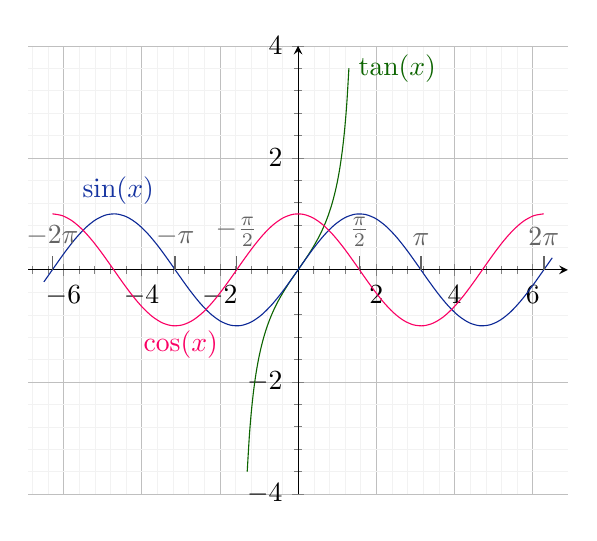
\begin{tikzpicture}
    \begin{axis}%
      [grid=both,
        minor tick num=4,
        grid style={line width=.1pt, draw=gray!10},
        major grid style={line width=.2pt,draw=gray!50},
        axis lines=middle,
        enlargelimits={abs=0.4}
      ]
      \addplot[domain=-1.3:1.3,samples=50,smooth,dg] {tan(deg(x))} node[right] {$\tan(x)$};
      \addplot[domain=-6.5:6.5,samples=50,smooth,db] {sin(deg(x))};
      \addplot[domain=-2*pi:2*pi,samples=50,smooth,dr] {cos(deg(x))};
      \node[dbt, above] at (axis cs:-4.6,1) {$\sin(x)$};
      \node[dr, above] at (axis cs:-3,-1.75) {$\cos(x)$};
      \draw[-, line width=0.2mm, dark] (pi,0) -- (pi,0.25) node[above] {$\pi$};
      \draw[-, line width=0.2mm, dark] (-pi,0) -- (-pi,0.25) node[above] {$-\pi$};
      \draw[-, line width=0.2mm, dark] (2*pi,0) -- (2*pi,0.25) node[above] {$2\pi$};
      \draw[-, line width=0.2mm, dark] (-2*pi,0) -- (-2*pi,0.25) node[above] {$-2\pi$};
      \draw[-, line width=0.1mm, dark] (pi/2,0) -- (pi/2,0.25) node[above] {$\frac{\pi}{2}$};
      \draw[-, line width=0.1mm, dark] (-pi/2,0) -- (-pi/2,0.25) node[above] {$-\frac{\pi}{2}$};
    \end{axis}
  \end{tikzpicture}
\end{center}



\subsection{Ableitungen}
\begin{center}
  % the c>{\centering\arraybackslash}X is a workaround to have a column fill up all space and still be centered
  \begin{tabularx}{\linewidth}{c>{\centering\arraybackslash}Xc}
    \toprule
    $\mathbf{F(x)}$                        & $\mathbf{f(x)}$          & $\mathbf{f'(x)}$               \\
    \midrule
    $\frac{x^{-a+1}}{-a+1}$                & $\frac{1}{x^a}$          & $\frac{a}{x^{a+1}}$            \\
    $\frac{x^{a+1}}{a+1}$                  & $x^a \ (a \ne -1)$       & $a \cdot x^{a-1}$              \\
    $\frac{1}{k \ln(a)}a^{kx}$             & $a^{kx}$                 & $ka^{kx} \ln(a)$               \\
    $\ln |x|$                              & $\frac{1}{x}$            & $-\frac{1}{x^2}$               \\
    $\frac{2}{3}x^{3/2}$                   & $\sqrt{x}$               & $\frac{1}{2\sqrt{x}}$          \\
    $\frac{n}{n+1}x^{\frac{1}{n}+1}$       & $\sqrt[n]{x}$            & $\frac{1}{n}x^{\frac{1}{n}-1}$ \\
    $-\cos(x)$                             & $\sin(x)$                & $\cos(x)$                      \\
    $\sin(x)$                              & $\cos(x)$                & $-\sin(x)$                     \\
    $\frac{1}{2}(x-\frac{1}{2}\sin(2x))$   & $\sin^2(x)$              & $2 \sin(x)\cos(x)$             \\
    $\frac{1}{2}(x + \frac{1}{2}\sin(2x))$ & $\cos^2(x)$              & $-2\sin(x)\cos(x)$             \\
    \multirow{2}*{$-\ln|\cos(x)|$}         & \multirow{2}*{$\tan(x)$} & $\frac{1}{\cos^2(x)}$          \\
                                           &                          & $1 + \tan^2(x)$                \\
    $\cosh(x)$                             & $\sinh(x)$               & $\cosh(x)$                     \\
    $\log(\cosh(x))$                       & $\tanh(x)$               & $\frac{1}{\cosh^2(x)}$         \\
    $\ln | \sin(x)|$                       & $\cot(x)$                & $-\frac{1}{\sin^2(x)}$         \\
    $\frac{1}{c} \cdot e^{cx}$             & $e^{cx}$                 & $c \cdot e^{cx}$               \\
    $x(\ln |x| - 1)$                       & $\ln |x|$                & $\frac{1}{x}$                  \\
    $\frac{1}{2}(\ln(x))^2$                & $\frac{\ln(x)}{x}$       & $\frac{1 - \ln(x)}{x^2}$       \\
    $\frac{x}{\ln(a)} (\ln|x| -1)$         & $\log_a |x|$             & $\frac{1}{\ln(a)x}$            \\
    \bottomrule
  \end{tabularx}
\end{center}
\subsection{Weitere Ableitungen}
\begin{center}
  \begin{tabularx}{\linewidth}{>{\centering\arraybackslash}X>{\centering\arraybackslash}X}
    \toprule
    $\mathbf{F(x)}$                                     & $\mathbf{f(x)}$                          \\
    \midrule
    $\frac{1}{a\cdot (n+1)}(ax+b)^{n+1}$                & $(ax+b)^n$                               \\

    $\arcsin(x)$                                        & $\frac{1}{\sqrt{1 - x^2}}$               \\
    $\arccos(x)$                                        & $\frac{-1}{\sqrt{1 - x^2}}$              \\
    $\arctan(x)$                                        & $\frac{1}{1 + x^2}$                      \\
    $\text{arcsinh}(x)$                                 & $\frac{1}{\sqrt{1 + x^2}}$               \\
    $\text{arccosh}(x) $                                & $\frac{1}{\sqrt{x^2 - 1}}$               \\
    $\text{arctanh}(x) $                                & $\frac{1}{1 - x^2}$                      \\
    $x^x \ (x > 0)$                                     & $x^x \cdot (1 + \ln x)$                  \\
    $\log_a|x|$                                         & $\frac{1}{x \ln a}=\log_a(e)\frac{1}{x}$ \\
    $\frac{(ax+b)^{n+2}}{a^2(n+1)(n+2)}$                & $\frac{(ax+b)^{n+1}}{a\cdot (n+1)}$      \\
    $\sqrt{1-x^2}+x\cdot \text{arcsin}(x)$              & $\arcsin(x)$                             \\
    $x\cdot \arccos(x)-\sqrt{1-x^2}$                    & $\arccos(x)$                             \\
    $x\cdot \arctan(x)-\frac{1}{2} \log(x^2+1)$         & $\arctan(x)$                             \\
    $x\cdot \text{arcsinh}(x)-\sqrt{x^2+1}$             & $\text{arcsinh}(x)$                      \\
    $x\cdot \text{arccosh}(x)-\sqrt{x^2-1}\sqrt{x^2+1}$ & $\text{arccosh}(x)$                      \\
    $\frac{1}{2} \log(1-x^2)+x\cdot \text{arctanh}(x)$  & $\text{arctanh}(x)$                      \\
    $\frac{\alpha}{\gamma}\log|\gamma x+\beta|$         & $\frac{\alpha}{\gamma x+\beta}$          \\
    \bottomrule
  \end{tabularx}
\end{center}

\subsection{Integrale}

\begin{center}
  \begin{tabularx}{\linewidth}{>{\centering\arraybackslash}X>{\centering\arraybackslash}X}
    \toprule
    $\mathbf{f(x)}$                      & $\mathbf{F(x)}$                                                  \\
    \midrule
    $\int f'(x) f(x) \dx$                & $\frac{1}{2}(f(x))^2$                                            \\
    $\int \frac{f'(x)}{f(x)} \dx$        & $\ln|f(x)|$                                                      \\
    $\int_{-\infty}^\infty e^{-x^2} \dx$ & $\sqrt{\pi}$                                                     \\
    $\int (ax+b)^n \dx$                  & $\frac{1}{a(n+1)}(ax+b)^{n+1}$                                   \\
    $\int x(ax+b)^n \dx$                 & $\frac{(ax+b)^{n+2}}{(n+2)a^2} - \frac{b(ax+b)^{n+1}}{(n+1)a^2}$ \\
    $\int (ax^p+b)^n x^{p-1} \dx$        & $\frac{(ax^p+b)^{n+1}}{ap(n+1)}$                                 \\
    $\int (ax^p + b)^{-1} x^{p-1} \dx$   & $\frac{1}{ap} \ln |ax^p + b|$                                    \\
    $\int \frac{ax+b}{cx+d} \dx$         & $\frac{ax}{c} - \frac{ad-bc}{c^2} \ln |cx +d|$                   \\
    $\int \frac{1}{x^2+a^2} \dx$         & $\frac{1}{a} \arctan \frac{x}{a}$                                \\
    $\int \frac{1}{x^2 - a^2} \dx$       & $\frac{1}{2a} \ln\left| \frac{x-a}{x+a} \right|$                 \\
    $\int \sqrt{a^2+x^2} \dx $           & $\frac{x}{2}f(x) + \frac{a^2}{2}\ln(x+f(x))$                     \\
    \bottomrule
  \end{tabularx}
\end{center}

\subsection{Definite Integrale}
\begin{center}
  $\int_0^{2\pi}\sin(x)=\int_0^{2\pi}\cos(x)=0$, \\$\int_0^{2\pi}\sin^2(x)=\int_0^{2\pi}\cos^2(x)=\pi$
\end{center}

\begin{subbox}{Gaußsche Glockenkurve}
  Für das uneigentliche Integral über die \textit{gaußsche Glockenkurve} gilt

  $$
    \int_{-\infty}^{\infty} e^{\frac{-x^{2}}{2 \sigma^{2}}} \mathrm{~d} x=\sqrt{2 \pi \sigma^{2}}
  $$
\end{subbox}


\clearpage

\renewcommand*{\arraystretch}{2}
\begin{center}

\subsection{Verteilungen}

  \begin{tabularx}{\textwidth}{|l|l|l|X|X|X|X|}
    \hline
    Verteilung               & Notation                                               & Parameter                                           & \( \E[X] \)                      & \( \Var(X) \)                                             & \( p_X(t)/f_X(t) \)                                                                                                                           & \( F_X(t) \)                                                               \\
    \hline
    \hline
    Gleichverteilung & unbekannt & \makecell[l]{\( n \): Anzahl Ereignisse                                                                                                   \\ (\( x_i \): Ereignisse)} & \( \frac{1}{n} \sum_{i=1}^{n} x_i \) & \( \frac{1}{n} \sum_{i=1}^{n} x_i^2 - \frac{1}{n^2} \left(\sum_{i=1}^{n} x_i \right)^2 \) & \( \frac{1}{n} \) & \( \frac{|\{k:x_k \leq t\}|}{n} \) \\
    \hline
    Bernoulli                & $\text{Ber}(p)$                                   & \( p: \) ErfolgsW'keit                              & \( p \)                          & \( p \cdot (1-p) \)                                       & \( p^t(1-p)^{1-t} \)                                                                                                                          & \( 1-p \) für \( 0 \leq t < 1 \)                                           \\
    \hline
    Binomial & $\text{Bin}(n,p)$        & \makecell[l] {\( n \): Anzahl Versuche                                                                                                    \\ \( p: \) ErfolgsW'keit } & \( np \) & \( np(1-p) \) & \( \binom{n}{t}p^t(1-p)^{n-t} \) & \( \sum_{k=0}^{t} \binom{n}{k} p^k(1-p)^{n-k} \)  \\
    \hline
    Geometrisch & $\text{Geo}(p)$     & \makecell[l] { \( p \): ErfolgsW'keit                                                                                                         \\ (\( t: \) Anzahl Versuche)} & \( \frac{1}{p} \) & \( \frac{1-p}{p^2} \) & \( p(1-p)^{t-1} \) & \( 1-(1-p)^t\) \\
    \hline
    Poisson&  $\text{Poisson}(\lambda)$   & \makecell[l]{ \( \lambda \): Erwartungswert                                                                                               \\ und Varianz} & \( \lambda \) & \( \lambda \) & \( \frac{\lambda^t}{t!}e^{-\lambda} \) & \( e^{-\lambda} \sum_{k=0}^{t} \frac{\lambda^{k}}{k!} \) \\
    \hline
    \makecell[l]{Gleichverteilung\\(im Intervall)} & $U \sim \mathcal{U}([0,1])$      & \( [a,b] \): Intervall               & \( \frac{a+b}{2} \)              & \( \frac{1}{12}(b-a)^2 \)        & \(\begin{cases} \frac{1}{b-a} &a \le x \le b \\ 0 & \text{sonst}\end{cases}\)                                                                                                                & \(\begin{cases} 0 & x\le a \\ \frac{t-a}{b-a} & a < x < b \\ 1 & x \ge b \end{cases}\)                \\
    \hline
    Exponentialv.            & $ \text{Exp}(\lambda)$                            & \( \lambda: \frac{1}{\E[X]} \)                      & \( \frac{1}{\lambda} \)          & \( \frac{1}{\lambda^2} \)                                 & \( \begin{cases} \lambda e^{-\lambda t} & t \geq 0 \\ 0 & t < 0 \end{cases} \)                                                                                                              & \( \begin{cases} 1-e^{-\lambda t} & t>0 \\ 0 & t \leq 0\end{cases}\)                                            \\
    \hline
    Normalverteilung & $\mathcal{N}\left(\mu, \sigma^2\right)$         & \makecell[l]{\( \mu: \E[X] \)                                                                                                                                                                                                                                                                       \\ \( \sigma^2 \): Varianz} & \( \mu \) & \( \sigma ^2 \) & \( \frac{1}{\sqrt{2\pi \sigma^2} }e^{-{\frac{(t-\mu)^2}{2\sigma^2} }} \) & \( \frac{1}{\sigma {\sqrt{2\pi}}} \int_{-\infty}^t e^{-\frac{1}{2}\left( \frac{y-\mu}{\sigma} \right) ^2} \mathrm{d} y \) \\
    \hline
    \( \chi ^2 \)-Verteilung & $\chi_{m}^{2}$                                    & \( n \): Freiheitsgrad                              & \( n \)                          & \( 2n \)                                                  & \( \frac{1}{2^{\frac{n}{2}}\Gamma (\frac{n}{2})} t^{\frac{n}{2}-1} e^{-\frac{t}{2}} \text{ für } t>0\)                                        & \(P\left( \frac{n}{2}, \frac{t}{2}\right) \)                               \\
    \hline
    t-Verteilung             & $t_{m}$                                         & \( n \): Freiheitsgrad                              & \( \begin{cases} 0 & n>1 \\ \text{undef.} & \text{sonst} \end{cases} \) & \( \begin{cases} \frac{n}{n-2} & n> 2 \\ \infty & 1<n \leq 2 \\ \text{undef.} & \text{sonst} \end{cases} \)                          & \( \frac{\Gamma \left( \frac{n+1}{2} \right) }{\sqrt{n\pi } \cdot \Gamma (\frac{n}{2})} \left( 1+ \frac{t^2}{n} \right) ^{- \frac{n+1}{2}} \) & zu kompliziert                                                             \\
    \hline
    Negativbinomial          & \(\operatorname{NBin}(r, p)\)                   & \(r \in \mathbb{N}\), \(p \in [0,1]\)               & $\frac{r}{p}$                    & $\frac{r(1-p)}{p^2}$                                      & $\binom{k-1}{r-1} p^r (1-p)^{k-r}$                                                                                                            & zu kompliziert                                                             \\
    \hline

    Cauchy-Verteilung        & $\operatorname{Cauchy}\left(x_0, \gamma\right)$ & \(x_0 \in \mathbb{R}\), \(\gamma > 0\)              & Existiert nicht                  & Existiert nicht                                           & \(\frac{1}{\pi} \frac{\gamma}{\gamma^2 + (x-x_0)^2}\)                                                                                         & \(\frac{1}{2} + \frac{1}{\pi} \arctan\left(\frac{x - x_0}{\gamma}\right)\) \\
    \hline

    Hypergeometrisch         & \(\mathrm{H}(n, r, m)\)                         & \(n \in \mathbb{N}\), \(m, r \in \{1, \ldots, n\}\) & $m\frac{r}{n}$                   & $m \frac{r}{n}\left(1-\frac{r}{n}\right) \frac{n-m}{n-1}$ & $\frac{\binom{r}{k} \binom{n-r}{m-k}}{\binom{n}{m}}$                                                                                          & $\sum_{y=0}^k \frac{\binom{r}{y} \binom{n-r}{m-y}}{\binom{n}{m}}$          \\
    \hline
  \end{tabularx}

\end{center}

\vspace*{-0.05cm}
\begin{subbox}{Binomischer Lehrsatz}
  \[(x + y)^n = \sum_{k = 0}^n  \binom{n}{k} x^{n-k}y^k \quad \text{mit:}\quad  \binom{n}{k}=\frac{n!}{k!(n-k)!}\]
\end{subbox}
\break
\vspace*{14.75cm}
\begin{subbox}{Geometrische Reihe}
  Für $\alpha<1$:
  $$\sum_{n=0}^{\infty}\alpha^{n}=\frac{1}{1-\alpha}$$
\end{subbox}
\vspace*{14.75cm}
\begin{subbox}{Cauchy Produkt}
  Falls $\sum_{n= 0}^\infty a_n$ und $\sum_{n = 0}^\infty b_n$ absolut konv, dann
  $$\sum_{n = 0}^\infty \sum_{k = 0}^n a_kb_{n-k} = \sum_{n = 0}^\infty \sum_{i+j = n} a_ib_j = \left(\sum_{n = 0}^\infty a_n\right) \cdot \left(\sum_{k = 0}^\infty b_k\right)$$
\end{subbox}

